\documentclass[twoside, 11pt]{exam}

\usepackage[T1]{fontenc}
\usepackage[utf8]{inputenc}
\usepackage[dutch]{babel}

\usepackage[font={small,sf},labelfont={bf},labelsep=endash]{caption}
\usepackage{fouriernc}
\usepackage[detect-all, binary-units, separate-uncertainty=true,
            per-mode=symbol, retain-explicit-plus, range-phrase={ tot },
            list-final-separator={ en }, output-decimal-marker={,}]
            {siunitx}

\usepackage{setspace}
\setstretch{1.2}

\setlength{\parskip}{\smallskipamount}
\setlength{\parindent}{0pt}

\usepackage{geometry}
\geometry{a4paper, vmargin=3cm, inner=3cm, outer=2cm, head=14pt}

\usepackage{float}

\usepackage[fleqn]{amsmath}
\numberwithin{equation}{section}
\numberwithin{figure}{section}

\usepackage{graphicx}
\graphicspath{{Figures/}}
\usepackage{subfig}

\usepackage[svgnames]{xcolor}
\usepackage{tikz}
\usepackage{tikz-3dplot}
\usepackage{pgfplots}
\usetikzlibrary{plotmarks,circuits.ee.IEC,pgfplots.groupplots,external,calc}
\pgfplotsset{compat=1.3}

\usepackage{minted}
\usepackage{amsthm}
\usepackage{relsize}
\usepackage{xspace}
\usepackage{url}
\usepackage{sansmath}
\usepackage{titling}


\theoremstyle{plain}
\newtheorem*{note}{Note}


\newcommand{\figref}[1]{Figuur~\ref{#1}}

\newcommand{\hisparc}{\textsmaller{HiSPARC}\xspace}
\newcommand{\kascade}{\textsmaller{KASCADE}\xspace}
\newcommand{\sapphire}{\textsmaller{SAPPHiRE}\xspace}
\newcommand{\jsparc}{\textsmaller{jSparc}\xspace}
\newcommand{\hdf}{\textsmaller{HDF5}\xspace}
\newcommand{\aires}{\textsmaller{AIRES}\xspace}
\newcommand{\csv}{\textsmaller{CSV}\xspace}
\newcommand{\python}{\textsmaller{PYTHON}\xspace}
\newcommand{\corsika}{\textsmaller{CORSIKA}\xspace}
\newcommand{\labview}{\textsmaller{LabVIEW}\xspace}
\newcommand{\dspmon}{\textsmaller{DSPMon}\xspace}
\newcommand{\daq}{\textsmaller{DAQ}\xspace}
\newcommand{\adc}{\textsmaller{ADC}\xspace}
\newcommand{\adcs}{\textsmaller{ADC}s\xspace}
\newcommand{\Adcs}{A\textsmaller{DC}s\xspace}
\newcommand{\hi}{\textsc{h i}\xspace}
\newcommand{\hii}{\textsc{h ii}\xspace}
\newcommand{\mip}{\textsmaller{MIP}\xspace}
\newcommand{\hisparcii}{\textsmaller{HiSPARC II}\xspace}
\newcommand{\hisparciii}{\textsmaller{HiSPARC III}\xspace}
\newcommand{\pmt}{\textsmaller{PMT}\xspace}
\newcommand{\pmts}{\textsmaller{PMT}s\xspace}
\newcommand{\gps}{\textsmaller{GPS}\xspace}

\DeclareSIUnit{\electronvolt}{\ensuremath{\mathrm{e\!\!\:V}}}

\DeclareSIUnit{\unitsigma}{\ensuremath{\sigma}}
\DeclareSIUnit{\mip}{\textsmaller{MIP}}
\DeclareSIUnit{\adc}{\textsmaller{ADC}}

\DeclareSIUnit{\gauss}{G}
\DeclareSIUnit{\parsec}{pc}
\DeclareSIUnit{\year}{yr}


%% Document style definitions

% macros and commands
\newcommand{\shorttitle}[1]{\def\theshorttitle{#1}}
\newcommand{\docindex}[1]{\def\thedocindex{#1}}
\newcommand{\version}[1]{\def\theversion{#1}}
\newcommand{\setsectionstyle}[2]{
  \colorlet{seccolor}{#1}
  \def\thesectiontitle{#2}
}

\newcommand{\setdocumentstyle}[4]{
  \setsectionstyle{#1}{#2}
  \docindex{#3}
  \shorttitle{#4}
}

% document types
\newcommand{\docalgemeen}[2]{\setdocumentstyle{red}{Algemeen}{#1}{#2}}
\newcommand{\docinstallatie}[2]{\setdocumentstyle{Gold}{Detector installatie}{#1}{#2}}
\newcommand{\docdetector}[2]{\setdocumentstyle{blue}{Detector}{#1}{#2}}
\newcommand{\docweerstation}[2]{\setdocumentstyle{LightSlateGray}{Weerstation}{#1}{#2}}
\newcommand{\docbliksem}[2]{\setdocumentstyle{orange}{Bliksem}{#1}{#2}}
\newcommand{\docanalyse}[2]{\setdocumentstyle{DarkViolet}{Data analyse}{#1}{#2}}
\newcommand{\docwerkblad}[2]{\setdocumentstyle{ForestGreen}{Werkbladen}{#1}{#2}}
\newcommand{\docdocent}[2]{\setdocumentstyle{DarkKhaki}{Uitwerkingen}{#1}{#2}}
\newcommand{\docopdrachten}[2]{\setdocumentstyle{Silver}{Opdrachten}{#1}{#2}}
\newcommand{\docrecept}[2]{\setdocumentstyle{Navy}{Recept}{#1}{#2}}

\pgfmathsetlengthmacro\stylemarginsep{+1cm}
\pgfmathsetlengthmacro\stylethumbsep{+.75cm}

\newcommand{\rightthumb}{
\begin{tikzpicture}[remember picture, overlay]
  % vertical line
  \draw[seccolor]
    ($(current page.north east) + (-\stylemarginsep, -.5cm)$) --
    ($(current page.south east) + (-\stylemarginsep, .5cm)$);

  % thumb
  \fill[seccolor]
    ($(current page.north east) +
      (-\stylemarginsep, -2cm -\thedocindex * \stylethumbsep)$)
      rectangle +(.5cm, -.5cm);
\end{tikzpicture}
}

\newcommand{\leftthumb}{
\begin{tikzpicture}[remember picture, overlay]
  % vertical line
  \draw[seccolor]
    ($(current page.north west) + (\stylemarginsep, -.5cm)$) --
    ($(current page.south west) + (\stylemarginsep, .5cm)$);

  % thumb
  \fill[seccolor]
    ($(current page.north west) +
      (\stylemarginsep, -2cm -\thedocindex * \stylethumbsep)$)
      rectangle +(-.5cm, -.5cm);
\end{tikzpicture}
}

\renewcommand{\maketitle}{
  \suppressfloats

  \begin{titlepage}
  \thispagestyle{\defaultstyle}
  \let\endtitlepage\relax
  \begin{tikzpicture}[remember picture, overlay,
    titlebox/.append style={seccolor, fill, text=white, minimum height=1cm,
      font=\sffamily\huge, draw=none},
    authorbox/.append style={minimum height=.5cm, font=\sffamily}]

    \node[titlebox, anchor=north west, shift={(3cm, -1cm)}] at
      (current page.north west) {\thesectiontitle};

    \node[anchor=north west, shift={(2.83cm, -2cm)}] at
      (current page.north west) {
\includegraphics[scale=.8]{../HiSPARC_header}};

    \node[titlebox, anchor=north east, shift={(-\stylemarginsep, -1cm)}] at
      (current page.north east) {\thetitle};

    \node[authorbox, anchor=north east, shift={(-\stylemarginsep, -2cm)}] at
      (current page.north east) {\theauthor};
  \end{tikzpicture}
  \end{titlepage}
}


\newcommand{\defaultstyle}{headandfoot}

% style definitions
\pagestyle{\defaultstyle}
\chead{\oddeven{\rightthumb}{\leftthumb}}
\cfoot{\theshorttitle\ -- \thepage}
\lfoot{\oddeven{}{\textcolor{gray}{\smaller Versie \theversion}}}
\rfoot{\oddeven{\textcolor{gray}{\smaller Versie \theversion}}{}}

\renewcommand{\thequestion}{\textbf{Opdracht \arabic{question}:}}
\renewcommand{\solutiontitle}{\noindent\textbf{Antwoord:}\enspace}
\newcommand{\makelines}[1]{\ifprintanswers\else\fillwithlines{#1\linefillheight}\fi}

\ifdefined\showanswers
  \printanswers
\else
  \noprintanswers
\fi


\usepackage{lipsum}

\title{HiSPARC Toegelicht} \author{C.G. van Veen} \docwerkblad{1}{HT}
\version{1.0}

\begin{document}

\maketitle

\section{Inleiding}

De aarde wordt continu gebombardeerd door kosmische straling. Dat zijn
deeltjes die uit het heelal vandaan komen zoals protonen, ijzerkernen en
koolstofkernen etc. Deze primaire deeltjes hebben energieën variërend
van \Si{10e2} t/m \Si{10e20} \electronvolt. De deeltjes met lagere
waarden voor energie zijn bijvoorbeeld deeltjes uitgezonden door de zon.
De deeltjes met hogere energiewaarden (>\Si{10e17} \electronvolt) hebben
een energie die we op aarde in versnellers niet kunnen bereiken. Het
noorderlicht ontstaat door deeltjes met een energie in de orde van een
keV, die op stikstof- en zuurstof moleculen botsen. Als primaire
deeltjes energieën hebben in de orde van \Si{10e14} t/m \Si{10e20}
\electronvolt en op atomen in de atmosfeer botsen ontstaat een lawine
van allerlei secundaire deeltjes \figref{fig:main_cosmicray_shower}, dat
een Extended Air Shower (EAS) wordt genoemd. Deze EAS reikt afhankelijk
van de energie van het primaire deeltje en de hoogte van de eerste
botsing tot het aardoppervlak. Victor Hess was de eerste die deze EAS of
kosmische showers daadwerkelijk gemeten heeft tijdens diverse metingen
met een luchtballon in 1912. Hess merkte dat de intensiteit van de
achtergrond straling hoger werd naarmate hij hoger in de atmosfeer kwam.
Men dacht toen straling voornamelijk uit de aarde afkomstig moest zijn
en de intensiteit dus zou moeten afnemen naar mate je verder van de
aarde af kwam. Tegenwoordig wordt er veel onderzoek verricht aan
kosmische straling en EAS, door onder andere de volgende
onderzoeksgroepen: KASCADE, AUGER. In Nederland is dit op scholen
mogelijk met HiSPARC.

\begin{figure} \centering
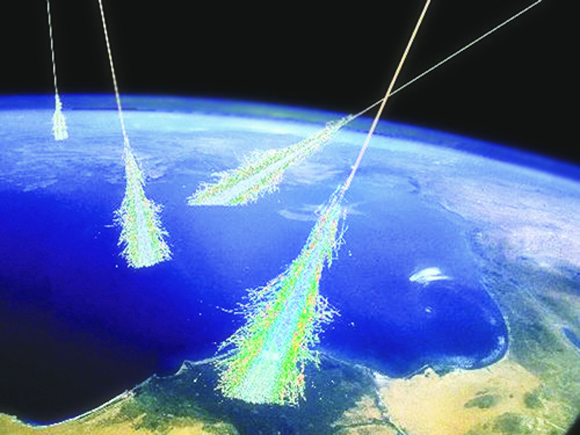
\includegraphics[scale=0.8]{main_cosmicray_shower} \caption{artiesten 
impressie van kosmische straling (bron: S. Swordy, Universiteit van
Chicago)} \label{fig:main_cosmicray_shower} \end{figure}

\Section{\hisparc}

Met dit Nederlandse project kunnen we EAS meten en analyseren. HiSPARC
is een samenwerking van middelbare scholen en universiteiten, waarbij de
scholen dienen als locatie waar de detectie stations geplaatst worden.
Leraren en leerlingen installeren, beheren en onderhouden de stations,
en houden de kwaliteit van de ermee verkregen meetgegevens in de gaten.
Zo worden EAS in een groot oppervlak gemeten en worden middelbare
scholieren betrokken bij wetenschappelijk onderzoek ondersteund door
universiteiten. Het doel van HiSPARC is om met behulp van de stations op
scholen onderzoek te doen aan deze kosmische showers. Onderzoeksvragen
met betrekking tot kosmische straling zijn, waar deze vandaan komen en
hoe ze ontstaan. De energie en richting zijn af te leiden uit de grootte
van de EAS en de tijdsverschillen in de detectoren. Waar kosmische
straling vandaan komt is gedeeltelijk bekend. Laag-energetische deeltjes
komen van de zon (de zonnewind) en van sterren uit ons melkwegstelsel.
Deeltjes met energieën tot ongeveer \Si{10e16} \electronvolt zijn
afkomstig van supernova's. Deeltjes met nog meer energie kunnen aan
magneetvelden van sterrenstelsels ontsnappen en zijn waarschijnlijk
buiten ons melkwegstelsel ontstaan. Hierbij denkt men aan een oorsprong
van primaire deeltjes uit Gamma-Ray Bursts (GRB), aan actieve kernen van
ver weg gelegen sterrenstelsels, en aan andere verschijnselen die met
zeer energetische plasmajets gepaard gaan. Kosmische straling kan
afkomstig zijn van zwarte gaten en actieve sterrenstelsels.

\section{Aantal kosmische showers}

Het aantal kosmische showers wat gemeten wordt, hangt sterk af van de
energie van het primaire deeltje. Primaire deeltjes met een 10 maal zo
hoge energie komen globaal 1000 maal zo weinig voor. In figuur 2 zie je
het diagram (op een dubbel logaritmische schaal) wat het overzicht geeft
tussen de flux (aantal showers per tijdseenheid per oppervlak) tegen de
energie van het primaire deeltje. Hierin is te zien dat het aantal
deeltjes met een energie van \Si{10e19} \electronvolt één keer per jaar
op een oppervlak van 1 \square\kilo\metre komt, door één \square\metre
gaat per seconde gemiddeld een deeltjes met een energie van \Si{10e11}
\electronvolt. Duidelijk is te zien dat de grafiek tussen \Si{10e20} t/m
\Si{10e21} \electronvolt ogenschijnlijk ophoudt. Deze grens wordt de
‘GZK cut-off’ genoemd. (Greisen–Zatsepin–Kuzmin limiet). Men vermoedt
dat de ‘GZK’ bovengrens vormt voor de energie van kosmische straling.
Zeker weten doen we dat niet omdat die energieën heel zeldzaam zijn.

\begin{figure} 
    \centering 
    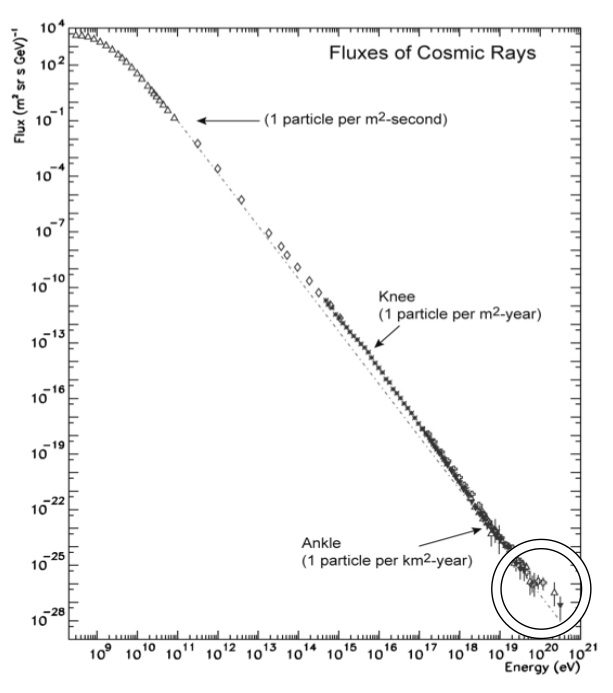
\includegraphics[scale=0.8]{swordy_blois}
    \caption{Flux als functie van de energie van kosmische straling. Tussen
    \Si{10e11} en \Si{10e15} \electronvolt meten we bijna geen flux omdat deeltjes met deze
energieën de grond niet bereiken. (bron: S. Swordy, Universiteit van
Chicago)} 
    \label{fig:swordy_blois} 
\end{figure}



\end{document}
